\section{Figure}

\begin{figure}[H]
  \centering
  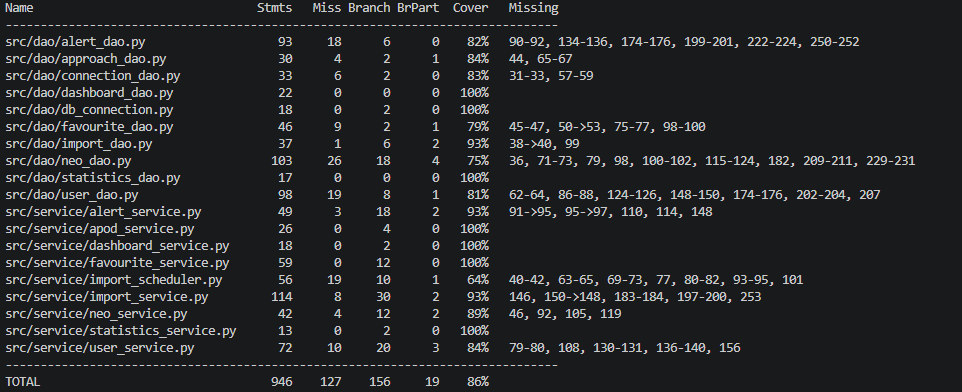
\includegraphics[width=0.95\textwidth]{figures/screenshot_tests.png}
  \caption{Detailed test coverage report}
  \label{fig:coverage}
\end{figure}

\section{Individual assessments}

\subsection{Mohammed-Adam Lakhrissi}

In this project, I was in charge of the dashboard (F2), the statistics (FO3) and the NASA Picture
of the Day with its export (FO8). For each of them, I wrote the whole chain, from the DAO to the
Streamlit page, including the unit tests. For the final report, I took care of the coordination
part: the title page, the introduction, the organization section and the conclusion.

At the beginning, the hardest part for me was to understand the layered architecture of the
template. To practise without risking breaking the team's code, I kept a personal copy of the
project where I redid the exercises of the practical sessions. After that, adding a new feature
became much more natural. The dashboard was the most difficult feature, because it depends on the
data of the other features.

Working with branches and pull requests on the same code base as three other people taught me a
lot, especially about keeping my changes small and clear so that they could be merged easily. I also started to see tests as useful rather than extra work, since they helped me
find mistakes in my own code.

Overall, I think the group worked well: the tasks were clearly split and it was easy to ask for
help. My workload was a bit lighter than that of the others, and I am grateful to my teammates for
taking this into consideration. I still tried to contribute as much as I could, both to the code
and to the reports. If I did the project again, I would test the whole application together earlier, since most
of our problems appeared at the end, when everything was connected.

\subsection{Yalalt Schneider}

During this work, my task was to implement features F5 and F6 related to Favourite and Alert. And I also did the first part of the import like preparing the tables, filling them with the data from NASA, and adding them to the app. But my teammates did the rest so that it would fit well in the app. 

Like everyone, I had to implement my features from the DAO to the Streamlit page. This allowed me to understand how an API works as during the first lesson I could barely distinguish the three layers. 

During the first week, this project seemed too big to me as there were plenty of details to think of before even starting to code. Finally, with the analysis report, it helped us to plan what we had to do and progress in the programme little by little.

But once the work started, the hardest part was the import. That was the first thing I did, and so it took a lot of time before being able to import data from NASA, understand the JSON responses, transfer them to the database. Each time I tried something, there was always one more error.

\bigskip

Altogether, I think that our group worked effectively, everyone knew what they should prepare and when it was due. But the thing that I appreciated the most is that everybody did their best, and so it was really easy to work. However, if I had to change one thing, it would be how we organized the end of the project. Probably, we started the final phase a bit too late, even though the deadline was still respected without being in a total hurry during the last day.


% --- The other members add their own assessment below ---
% \subsection{Sofia Bounaga}
% \subsection{Valentin Denni}